\documentclass{../../meta/tudscript}
\begin{document}
 \ssect{RSA-Verschlüsselung (Rivest, Shamir, Asleman, 1978)}
  Assymetrischs Public-Key-Kryptosystem mit zwei Arten von Schlüsseln. Einen öffentlichen zum Verschlüsseln und einen geheimen zum Entschlüsseln.\\
  
  Seien $p, q \in \bP, p \neq q$ und sei $n := p \cdot q$.\\
  Dann ist $\varphi (n) = (p-1) \cdot (q-1)$.\\
  Weiter $e, d \in \bZ$ mit $ed \equiv 1 \mod \varphi (n)$, d.h.
  \begin{flalign*}
  	[e]_{\varphi (n)} \in \bZ_{\varphi (n)}^* \text{mit} [e]_{\varphi (n)}^{-1} = [d]_{\varphi (n)}
end{flalign*}

  Öffentlicher Schlüssel: $k_p = (n, e)$\\
  	
  Geheimer Schlüssel: $k_s = (n, d)$\\
  
  Verfahren: Ist $m \in \bZ_n$ eine geheime Nachricht für Bob, so schickt er Alice den Chiffretext:
  \begin{flalign*}
  	c := m^e \in \bZ_n
  \end{flalign*}
  öffentlich an Bob.\\
  Diesen entschlüsselt Bob durch Berechnung
  \begin{flalign*}
  	\tilde{m} := c^d \in \bZ_n
  \end{flalign*}
  \underline{Behauptung}: $m = \tilde{m} (\in \bZ_n)$
  \sssect*{Beweis}
   Zunächst gilt (1):
   \begin{flalign*}
   	p|(m^{ed} - m)
   \end{flalign*}
   
   Beweis von (1): Ist $p|m$, dann $p|(m^{ed} - m)$ nach Proposition 9.2,2.\\
   Angenommen, p teilt m \underline{nicht}, d.h.:
   \begin{flalign*}
   	ggT(p, m) = 1
   \end{flalign*}
   Sei $k \in \bZ$ mit $ed = k \cdot \varphi (n) + 1 = k (p-1)(q-1)+1$.\\
   Nach Folgerung 11.16 (kleiner Satz von Fermat):
   \begin{flalign*}
   	m^{ed} = (\underbrace{m^{p-1}}_{\equiv 1 \mod p})^{k(q-1)} \cdot m \equiv m \mod p
   \end{flalign*}
   d.h. $p|(m^{ed} -m)$ Das beweist (1). Analog zeigt man (2)
   \begin{flalign*}
   	q|(m^{ed} - m)\hfill
   \end{flalign*}
   Aus (1) und (2) folgt mit Lemma 11.26:
   \begin{flalign*}
   	n = pq | (m^{ed} -m)
   \end{flalign*}
   d.h. $\tilde{m} = c^d = (m^e)^d = m^{ed} \equiv m \mod n \hfill\square$\\
   
   Die Sicherheit des RSA-Verfahrens basiert auf der Schwierigkeit, zum (öffentlich) gegebenen n die Primfaktoren p und q bestimmen (praktische äquivalent zur Bestimmung von $\varphi (n)$, siehe Lemma 12.7 unten).\\
   Ist dann $\varphi (n) = (p-1) (q-1)$ bekannt, so kann man aus dem öffentlichen Schlüssel e leicht (mit euklidischen Aldorithmus) 
  	den geheimen Schlüssel\\
  	$d \equiv e^{-1} \in \bZ_{\varphi (n)}^*$ zu bestimmen.
 
 \ssect{Lemma}
  Seien $p, q \in \bP, p \neq q$ und $n := pq$. Dann sind p und q die Nullstellen der Funktion
  \begin{flalign*}
  	f: \bZ \rightarrow \bZ, x \mapsto x^2 - (n - \varphi (n) + 1) \cdot x + n
  \end{flalign*}
  Genauer: $f(x) = (x-p)(x-q)$ für alle $x \in \bZ$
  
  \sssect*{Beweis}
   Nach Bemerkung 9.26 gilt:
   \begin{flalign*}
   	\varphi (n) = (p-1)(q-1) = pq - p -q + 1 = n - (p + q) + 1
   \end{flalign*}
   also $p + q = n - \varphi (n) + 1$. Damit für alle $x \in \bZ$:
   \begin{flalign*}
   	(x-p)(x-q) = x^2 - (p+q)x + pq = x^2 - (n- \varphi (n) + 1)x + n = f (x)\\
   	\hfill\square
   \end{flalign*}

\sect{Graphen}
 Für eine Menge $M$ sei
 \begin{flalign*}
 	\binom{M}{2} := \mathscr{P}_2 (M) := \Set{B \subseteq M \mid B \text{ endlich}, |B| = 2}
 \end{flalign*}
 
 \ssect{Definition: Graph}
  Ein \underline{Graph} ist ein Paar $G = (V, E)$\\
  bestehend aus einer Menge V und einer Menge $E \subseteq \binom{M}{2}$.\\
  Die Elemente von V heißen die \underline{Knoten/Ecken (engl. vertices)} und\\
  die Elemente von E heißen \underline{Kanten (engl. edges)} des Graphen G.\\
  Zwei Knoten $v, w \in V$ heißen \underline{benachbart/adjazent} in G, falls $\set{v, w} \in E$\\
  Der Graph G heiß \underline{endlich}, falls V (und damit auch E) endlich ist.
 \ssect{Beispiele}
  \begin{enumerate}
   \item Für $n \in \bN \setminus \Set{0}$ heißt
    \begin{flalign*}
    	K_n := (\underbrace{[n]}_{ = \set{1, \ldots, n}}, \binom{[n]}{2})
    \end{flalign*}
    \underline{vollständiger Graph (Clique)} auf n Knoten.\\
    Der Graph $K_n$ hat $\frac{1}{2}n \cdot (n-1)$ Knoten.\\
    
	Hier $K_5$ als Beispiel:
	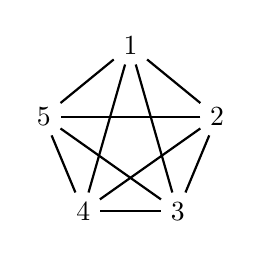
\begin{tikzpicture}
		\node at (0, 1.5) (5) {1};
		\node at (1.1, 0.6) (1) {2};
		\node at (0.6, -0.6) (2) {3};
		\node at (-0.6, -0.6) (3) {4};
		\node at (-1.1, 0.6) (4) {5};
		\draw [black,  thick] (1) -- (2);
		\draw [black,  thick] (2) -- (3);
		\draw [black,  thick] (3) -- (4);
		\draw [black,  thick] (4) -- (5);
		\draw [black,  thick] (5) -- (1);
		\draw [black,  thick] (1) -- (3);
		\draw [black,  thick] (1) -- (4);
		\draw [black,  thick] (5) -- (2);
		\draw [black,  thick] (5) -- (3);
		\draw [black,  thick] (4) -- (2);
	\end{tikzpicture}
	
   \item Für $n \in \bN \setminus \set{0}$ heißt
    \begin{flalign*}
    	C_n := ([n], \Set{\{i,j\} \mid i, j \in [n], j \equiv i + 1 \mod n})
    \end{flalign*}
    Kreis auf n Knoten (und n Kanten)\\
    
	Hier $C_5$ als Beispiel:
	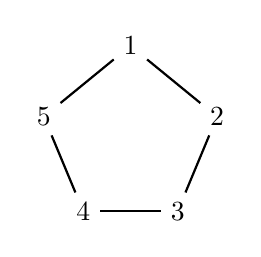
\begin{tikzpicture}
		\node at (0, 1.5) (5) {1};
		\node at (1.1, 0.6) (1) {2};
		\node at (0.6, -0.6) (2) {3};
		\node at (-0.6, -0.6) (3) {4};
		\node at (-1.1, 0.6) (4) {5};
		\draw [black,  thick] (1) -- (2);
		\draw [black,  thick] (2) -- (3);
		\draw [black,  thick] (3) -- (4);
		\draw [black,  thick] (4) -- (5);
		\draw [black,  thick] (5) -- (1);
	\end{tikzpicture}
    
   \item Sei $X := [5] = \Set{1, 2, 3, 4, 5}$.\\
    Der \underline{Petersen-Graph} $G = (V, E)$\\
    hat die Knottenmenge $V := \binom{X}{2}$\\
    und die Knotenmenge $E := \Set{\Set{A, B} \mid A, B \in \binom{X}{2}, A \cap B = \emptyset}$\\
	\begin{tikzpicture}
		\node at (0, 1.5) (12) {12};
		\node at (1.1, 0.6) (51) {51};
		\node at (0.6, -0.6) (45) {45};
		\node at (-0.6, -0.6) (34) {34};
		\node at (-1.1, 0.6) (23) {23};
		\draw [black,  thick] (1) -- (3);
		\draw [black,  thick] (1) -- (4);
		\draw [black,  thick] (5) -- (2);
		\draw [black,  thick] (5) -- (3);
		\draw [black,  thick] (4) -- (2);
		\node at (0, 3) (35) {35};
		\node at (2.6, 1.2) (24) {24};
		\node at (1.5, -1.8) (13) {13};
		\node at (-1.5, -1.8) (25) {25};
		\node at (-2.6, 1.2) (14) {14};
		\draw [black,  thick] (35) -- (24);
		\draw [black,  thick] (24) -- (13);
		\draw [black,  thick] (13) -- (25);
		\draw [black,  thick] (25) -- (14);
		\draw [black,  thick] (14) -- (35);
		\draw [black,  thick] (35) -- (12);
		\draw [black,  thick] (24) -- (51);
		\draw [black,  thick] (13) -- (45);
		\draw [black,  thick] (25) -- (34);
		\draw [black,  thick] (14) -- (23);
	\end{tikzpicture}
  \end{enumerate}
 
 \ssect{Definition: regulärer Graph}
  Sei $G = (V, E)$ endlicher Graph.\\
  Der \underline{Grad} eines Knotens $v \in V$ in G ist
  \begin{flalign*}
  	deg_G (v) :&= |\Set{w \in V \mid (v, w) \in E}|\\
  	&= |\Set{e \in E \mid v \in e}|
  \end{flalign*}
  Für $k \in \bN$ heißt G \underline{k-regulär}, falls $deg_G (v) = k$ für alle $v \in V$.\\
 G heißt \underline{regulär} $:\iff \exists k \in \bN:$ G k-regulär.
  
\end{document}
